\documentclass[../manuale-utente.tex]{subfiles}

\begin{document}

\subsection{Requisiti}%
\label{sub:web_app_requisiti}

\begin{description}
    \item[Browser:] Google Chrome 72.x, Firefox 65.x, Edge 44.x.
    \item[Necessario:] JavaScript.
\end{description}


\subsection{Manuale d'uso}%
\label{sub:manuale-uso-web}

\subsubsection{Pagina principale}%
\label{subs:pagina_principale}

\begin{figure}[H]
    \centering
    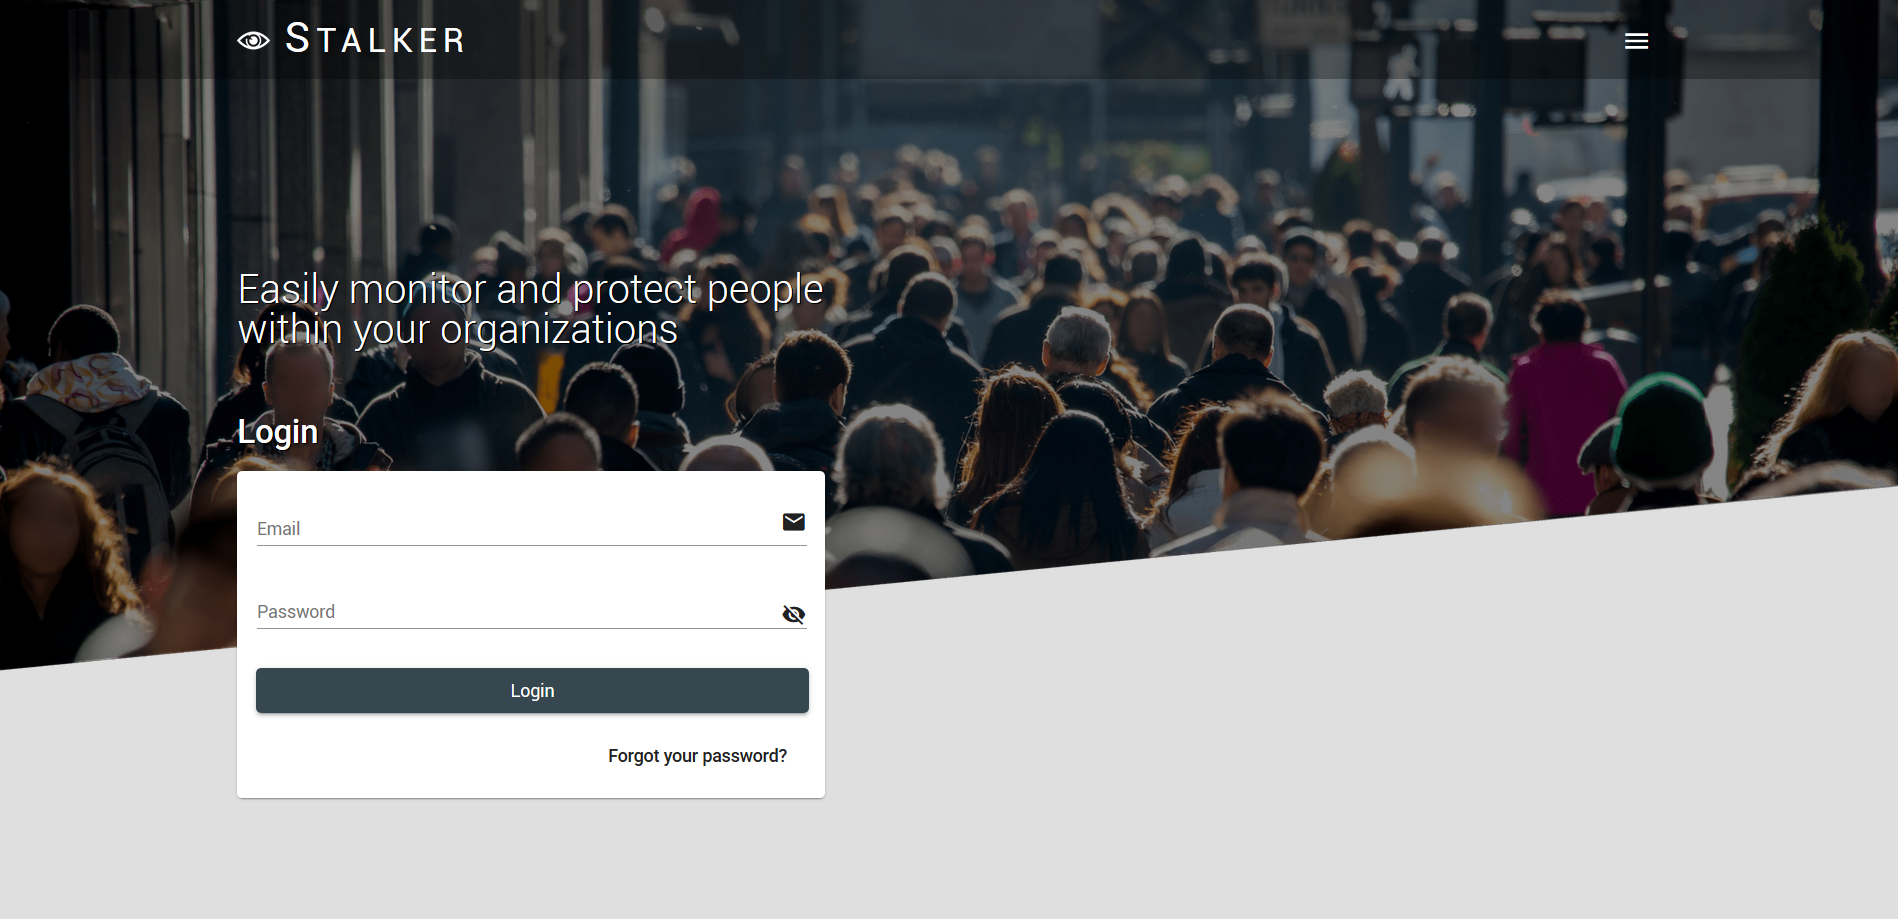
\includegraphics[width=175mm]{pagina-home.png}
    \caption{Pagina principale}%
    \label{fig:web_app_pagina_principale}
\end{figure}
Quando l'utente si vuole connettere all'interfaccia amministratore di Stalker, non è autenticato e può eseguire queste azioni, ognuna diversa dall'altra:
\begin{itemize}
    \item accedere a Stalker, nel caso sia già registrato, con le proprie credenziali email e password (paragrafo §~\ref{par:accesso_alla_web_application}).
    \item recuperare la password nel caso l'abbia smarrita (paragrafo §~\ref{par:recupero_password}).
    \item selezionare il menu ad hamburger posizionato sulla barra superiore a destra, per visualizzare le informazioni riguardo a Stalker. Questo menu è presente in ogni pagina.
\end{itemize}

\paragraph{Accesso alla web application}%
\label{par:accesso_alla_web_application}

\begin{figure}[H]
    \centering
    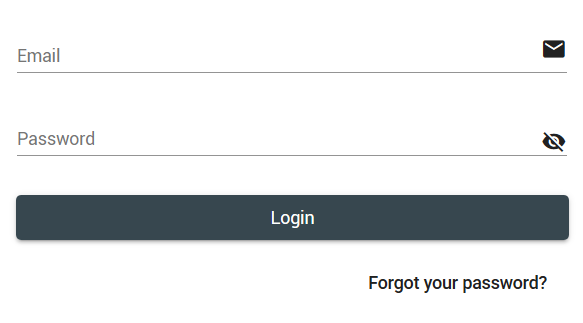
\includegraphics[width=120mm]{accesso-web-app.png}
    \caption{Form di accesso alla web application di Stalker}%
    \label{fig:web_app_form_accesso}
\end{figure}
L'utente vuole accedere al sistema di Stalker, quindi deve eseguire i seguenti passaggi:
\begin{itemize}
    \item inserire correttamente l'email.
    \item inserire la password. La password può essere visualizzata normalmente durante la sua digitazione, cliccando sull'occhio barrato alla fine del campo d'inserimento.
    \item selezionare il pulsante \textbf{Login} per concludere la procedura di accesso.
\end{itemize}
Nel caso l'operazione venga svolta correttamente, si avrà diritto all'accesso nella web application di Stalker, visualizzando la pagina del profilo personale (figura §~\ref{fig:web_app_visualizzazione_profilo_personale}).
In caso contrario, l'utente non è autorizzato, in quanto la procedura è fallita.
Le cause possono essere le seguenti:
\begin{itemize}
    \item l'email inserita non rispetta i vincoli imposti dal sistema di Stalker.
    \item la password non rispetta i vincoli imposti dal sistema di Stalker.
    \item l'email e la password inserite non rispettano i vincoli imposti dal sistema di Stalker.
    \item l'email e la password inserite rispettano i vincoli, ma non sono presenti all'interno del database di Stalker.
\end{itemize}
In ogni caso, il messaggio di errore non sarà specifico ma generico, per motivi di sicurezza.

\paragraph{Recupero password}%
\label{par:recupero_password}

\begin{figure}[H]
    \centering
    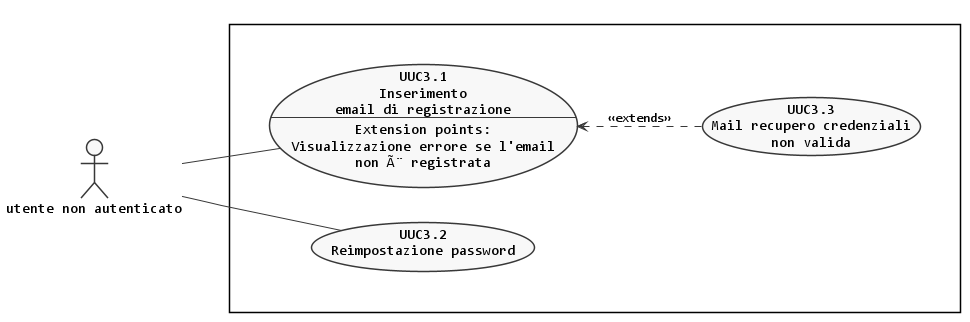
\includegraphics[width=150mm]{recupero-password.png}
    \caption{Form recupero password}%
    \label{fig:web_app_form_recupero_password}
\end{figure}
L'utente ha smarrito la password o non se la ricorda più, quindi deve eseguire tre passaggi:
\begin{itemize}
    \item cliccare alla voce \textbf{Forgot your password?} presente nel form per l'accesso alla web application (figura §~\ref{fig:web_app_pagina_principale}).
    \item inserire correttamente l'email.
    \item selezionare il pulsante \textbf{Recover} per inviare la richiesta al server.
\end{itemize}

Nel caso l'operazione venga svolta correttamente, la vecchia password verrà resettata e l'utente riceverà una mail sulla propria casella postale contenente la nuova password provvisoria che dovrà utilizzare al prossimo accesso in Stalker.
In caso contrario, l'utente non può recuperare la password, in quanto la procedura è fallita.
Le cause possono essere le seguenti:
\begin{itemize}
    \item l'email inserita non rispetta i vincoli imposti dal sistema di Stalker.
    \item l'email inserita rispetta i vincoli, ma non è presente nel database di Stalker, quindi non si può avviare la procedura.
\end{itemize}
In ogni caso, il messaggio di errore non sarà specifico ma generico, per motivi di sicurezza.

\subsubsection{Visualizzazione profilo personale}%
\label{subs:visualizzazione_profilo_personale}

\begin{figure}[H]
    \centering
    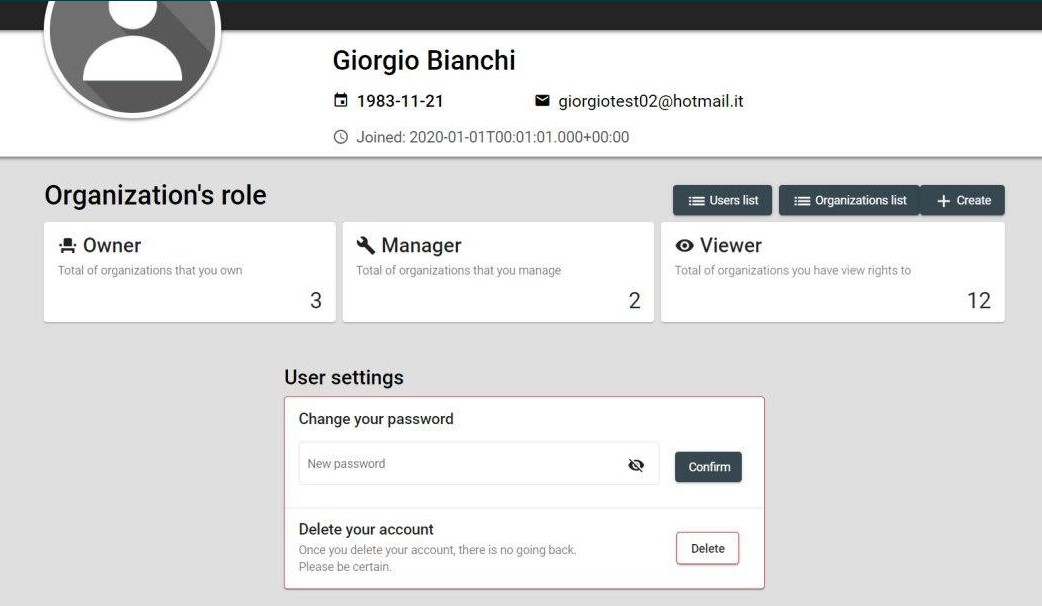
\includegraphics[width=170mm]{visualizza-profilo-personale.jpg}
    \caption{Visualizzazione profilo personale}%
    \label{fig:web_app_visualizzazione_profilo_personale}
\end{figure}
L'utente ha appena effettuato l'autenticazione alla web application di Stalker, quindi si ritrova nella pagina del profilo personale.
I dati che la pagina mette a disposizione dell'utente sono:
\begin{itemize}
    \item nome e cognome.
    \item la data di nascita.
    \item l'email con la quale è registrato in Stalker.
    \item data e ora in cui l'utente è stato aggiunto in Stalker.
    \item un'insieme di dati relativi ai ruoli che l'utente possiede in alcune delle organizzazioni di Stalker.
    \begin{itemize}
        \item il numero totale di organizzazioni in cui è owner.
        \item il numero totale di organizzazioni in cui è manager.
        \item il numero totale di organizzazioni in cui è viewer.
    \end{itemize}
\end{itemize}
Inoltre, la seguente pagina fornisce le seguenti operazioni:
\begin{itemize}
    \item la visualizzazione della lista di tutti gli utenti di Stalker, cliccando il pulsante \textbf{Users list} (sotto-sezione §~\ref{subs:visualizzazione_utenti}).
    \item la visualizzazione della lista di tutte le organizzazioni, cliccando il pulsante \textbf{Organizations list} (sotto-sezione §~\ref{subs:visualizzazione_organizzazioni}).
    \item la creazione di una nuova organizzazione, cliccando il pulsante \textbf{Create} (sotto-sezione §~\ref{subs:creazione_organizzazione}).
\end{itemize}
Infine, l'utente ha la possibilità di effettuare le seguenti operazioni sull'account personale di Stalker nel form \textit{User settings}:
\begin{itemize}
  \item cambiare la propria password per l'accesso a Stalker, inserendo quella nuova nella casella di input indicata con il \glossarioLocale{placeholder} \textit{New password} (con la possibilità di visualizzarla in chiaro cliccando l'occhio barrato) e cliccando il pulsante \textbf{Confirm}.
  \item eliminare il proprio account di Stalker, cliccando il pulsante \textbf{Delete}.
\end{itemize}
In entrambi i casi uscirà un \glossarioLocale{pop-up} per confermare o annullare l'operazione.

\subsubsection{Visualizzazione utenti}%
\label{subs:visualizzazione_utenti}

\begin{figure}[H]
    \centering
    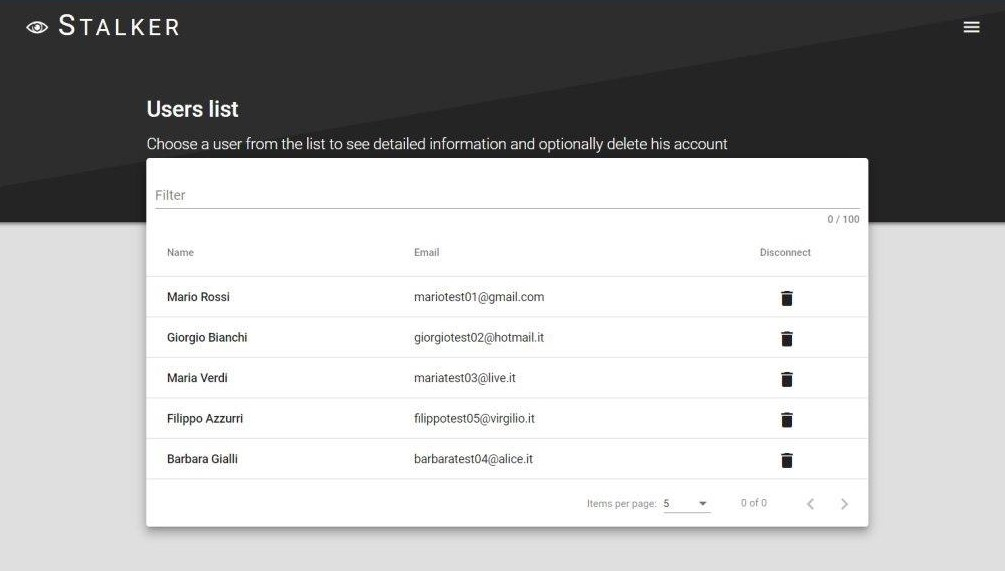
\includegraphics[width=160mm]{visualizza-utenti.jpg} %FIXME cambia immagine: colonna Disconnect sbagliata
    \caption{Visualizzazione utenti}%
    \label{fig:web_app_visualizzazione_utenti}
\end{figure}
L'utente ha cliccato il pulsante \textbf{Users list}, e quindi ha la possibilità di visualizzare la lista di tutti gli utenti registrati in Stalker.
La lista degli utenti contiene le seguenti informazioni:
\begin{description}
  \item[Name:] nome e cognome dell'utente.
  \item[Email:] email dell'utente.
\end{description}
L'utente ha la possibilità di interagire con la pagina e può eseguire queste operazioni:
\begin{itemize}
  \item selezionare un'utente specifico per accedere al suo profilo personale %TODO Inserire img pagina
  \item eliminare un'utente da Stalker, cliccando il pulsante a forma di bidone posto sotto la colonna \textbf{Delete}. Una volta cliccato, uscirà un pop-up nella quale verrà richiesto di confermare l'operazione inserendo la mail dell'utente da eliminare: in caso affermativo l'utente verrà eliminato, altrimenti non è consentita l'operazione di eliminazione. %TODO Inserire img dialog?
  \item filtrare gli utenti in lista per nome e cognome tramite un'apposita area di ricerca indicata con il placeholder \textit{Filter}, sopra la lista degli utenti.
  \item filtrare il numero di utenti visualizzabili in una pagina, tramite la tendina \textit{Items per page} sotto la lista degli utenti.
  \item cambiare la pagina della lista degli utenti, tramite le apposite frecce direzionali sotto la lista degli utenti.
\end{itemize}

\subsubsection{Visualizzazione organizzazioni}%
\label{subs:visualizzazione_organizzazioni}

\begin{figure}[H]
    \centering
    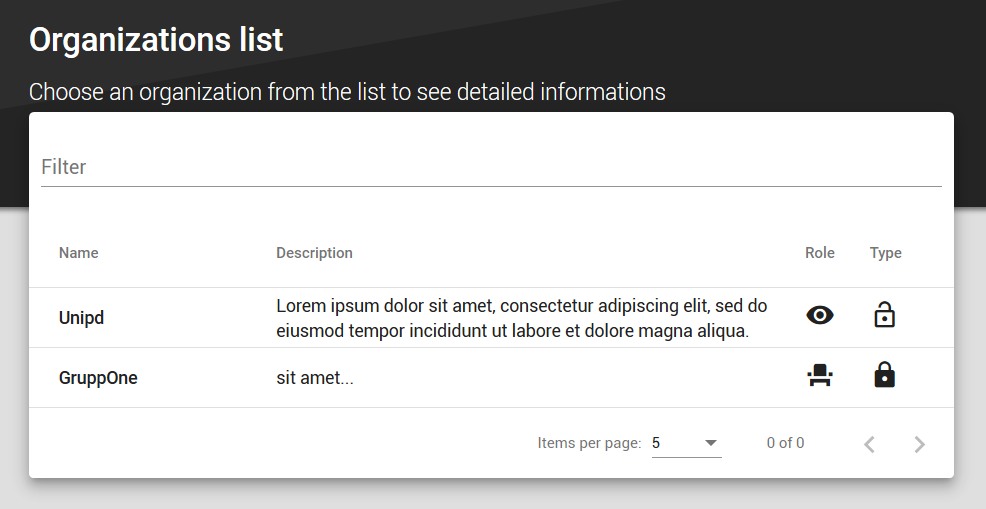
\includegraphics[width=180mm]{organizations-list.png}
    \caption{Visualizzazione organizzazioni}%
    \label{fig:web_app_visualizzazione_organizzazioni}
\end{figure}
L'utente ha cliccato il pulsante \textbf{Organizations list}, e quindi ha la possibilità di visualizzare la lista delle organizzazioni nelle quali ha un determinato ruolo.
La lista delle organizzazioni che l'utente visualizza contiene le seguenti informazioni:
\begin{description}
    \item[Name:] nome dell'organizzazione.
    \item[Description:] descrizione dell'organizzazione.
    \item[Role:] un'icona che rappresenta il ruolo dell'utente in un'organizzazione. È possibile visualizzare testualmente il ruolo di un utente spostando il cursore sopra l'icona.
    \item[Type:] un'icona che rappresenta se l'organizzazione è di dominio pubblico o di dominio privato: è possibile visualizzare testualmente il dominio di un'organizzazione spostando il cursore sopra l'icona.
\end{description}
L'utente ha la possibilità di interagire con la pagina e può eseguire queste operazioni:
\begin{itemize}
\item visualizzare la pagina della relativa organizzazione, contenente informazioni più dettagliate, cliccando sopra l'apposita organizzazione in lista.
\item filtrare le organizzazioni in lista per nome tramite un'apposita area di ricerca indicata con il placeholder \textit{Filter}, sopra la lista delle organizzazioni.
\item filtrare il numero di organizzazioni visualizzabili in una pagina, tramite la tendina \textit{Items per page} sotto la lista delle organizzazioni.
\item cambiare la pagina della lista delle organizzazioni, tramite le apposite frecce direzionali sotto la lista delle organizzazioni.
\end{itemize}

\paragraph{Visualizzazione dettagli organizzazione}%
\label{par:visualizzazione_dettagli_organizzazione}

\begin{figure}[H]
    \centering
    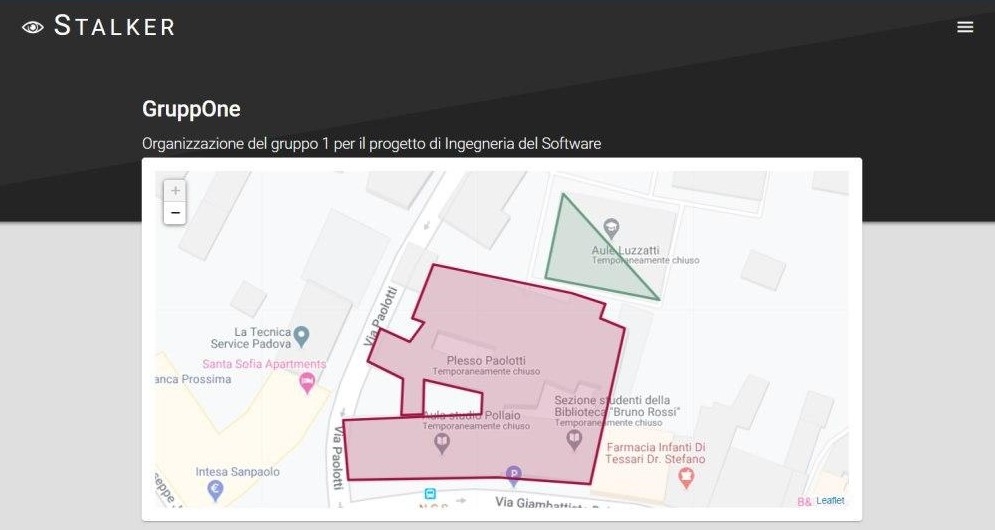
\includegraphics[width=180mm]{visualizza-dettagli-organizzazione-1.jpg}
    \caption{Visualizzazione dettagli organizzazione~- 1}%
    \label{fig:web_app_visualizzazione_dettagli_organizzazione-1}
\end{figure}
Una volta che l'utente seleziona un'organizzazione dalla lista di organizzazioni, viene indirizzato in un'altra pagina che riporta i dettagli dell'organizzazione selezionata.
La pagina contiene le seguenti informazioni:
\begin{itemize}
  \item il nome dell'organizzazione.
  \item una descrizione relativa all'organizzazione.
  \item una mappa, che può essere ingrandita o rimpicciolita, che contiene tutti i luoghi che appartengono all'organizzazione, evidenziati con colori diversi in modo da differenziarli chiaramente sulla mappa.
  \begin{figure}[H]
    \centering
    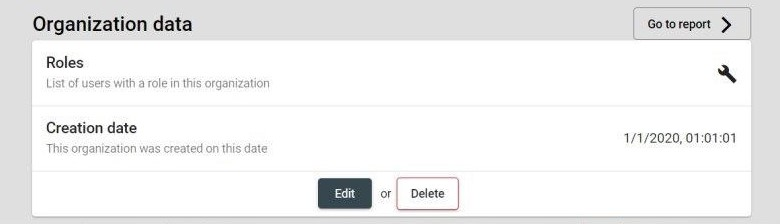
\includegraphics[width=180mm]{visualizza-dettagli-organizzazione-2.jpg}
    \caption{Visualizzazione dettagli organizzazione~- 2}%
    \label{fig:web_app_visualizzazione_dettagli_organizzazione-2}
  \end{figure}
  \item solo se l'organizzazione è privata, è presente la voce \textbf{LDAP Configuration} che indica i dati di configurazione del \glossarioLocale{server LDAP}.
  \item alla voce \textbf{Roles}, la lista degli utenti che hanno un ruolo nell'organizzazione, accessibile cliccando sul pulsante a forma di chiave inglese. %TODO Inserire img degli utenti con roles
  \item alla voce \textbf{Creation date}, la data e ora di creazione dell'organizzazione.
\end{itemize}
L'utente ha la possibilità di interagire con la pagina e può eseguire queste operazioni:
\begin{itemize}
  \item modificare le informazioni dell'organizzazione cliccando il pulsante \textbf{Edit}, venendo così indirizzati alla pagina di modifica (sotto-sezione §~\ref{subs:modififica_dettagli_organizzazione}). La modifica di questi dati è consentita solo agli utenti che ne hanno il diritto.
  \item eliminare l'organizzazione cliccando il pulsante \textbf{Delete}. Una volta cliccato, uscirà un pop-up per confermare o annullare l'operazione.
  \item visualizzare il report dell'organizzazione cliccando il pulsante \textbf{Go to report} (sotto-sezione §~\ref{subs:visualizza_report_organizzazione}).
\end{itemize}

\subsubsection{Creazione organizzazione}%
\label{subs:creazione_organizzazione}

L'utente vuole creare un'organizzazione, che avviene in 4 passaggi sequenziali.
I 4 passaggi per la creazione sono i seguenti:
\begin{enumerate}
    \item \textbf{Organization details}

    \begin{figure}[H]
      \centering
      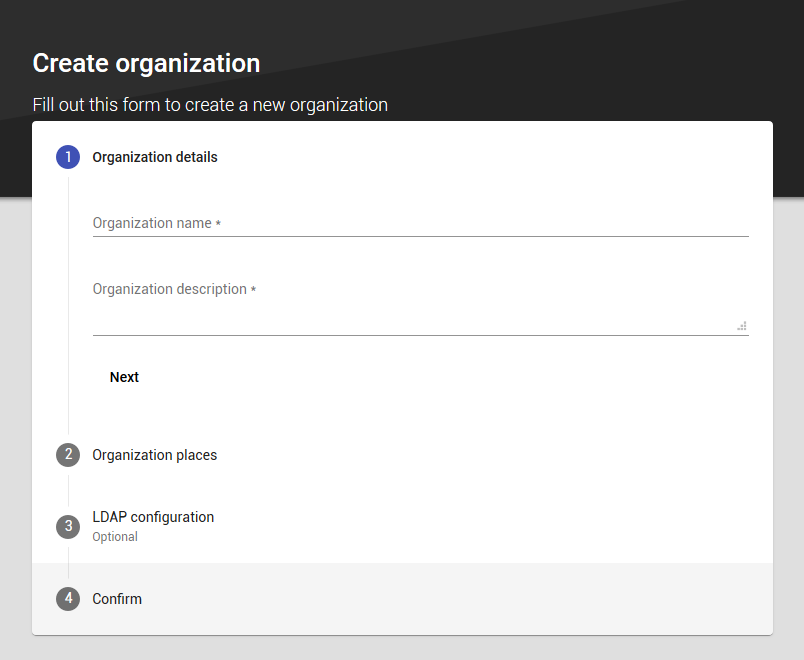
\includegraphics[width=120mm]{create-organization-1.png}
      \caption{Inserimento dettagli dell'organizzazione}%
      \label{fig:web_app_inserimento_dettagli_organizzazione}
    \end{figure}
    I campi che devono essere inseriti obbligatoriamente sono:
    \begin{description}
      \item[Organization name:] che corrisponde al nome dell'organizzazione che l'utente vuole creare.
      \item[Organization description:] che corrisponde alla descrizione dell'organizzazione che l'utente vuole creare.
    \end{description}
    Cliccando \textbf{Next} si va al passaggio 2.

    \item \textbf{Organization places}

    \begin{figure}[H]
      \centering
      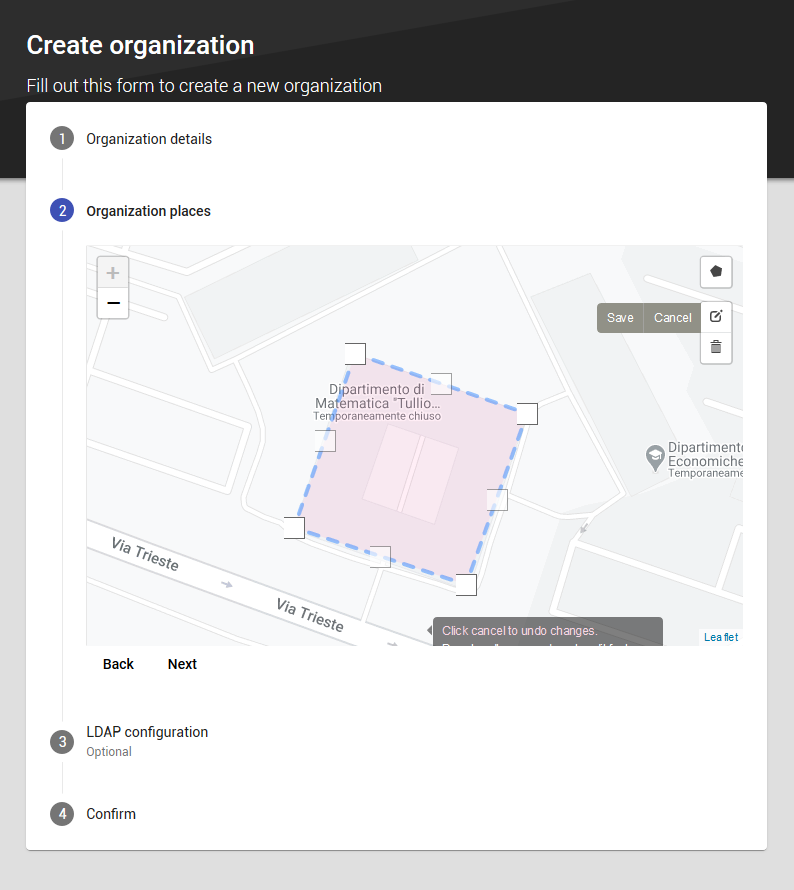
\includegraphics[width=120mm]{create-organization-2.png}
      \caption{Inserimento luoghi dell'organizzazione}%
      \label{fig:web_app_inserimento_luoghi_organizzazione}
    \end{figure}
    I luoghi si possono aggiungere direttamente dalla mappa interattiva, che si può ingrandire oppure rimpicciolire tramite i pulsanti in alto alla sinistra nella mappa.
    I luoghi si possono anche modificare oppure eliminare, nel caso in cui i luoghi creati siano errati.
    Per compiere azioni sulla mappa, ci sono tre pulsanti in alto a destra:
    \begin{itemize}
        \item cliccando il pulsante indicato con il poligono nero, si può creare un luogo bidimensionale sulla mappa cliccando con il tasto sinistro sui punti d'interesse. Per chiudere il poligono basta cliccare sul lato più adiacente all'ultimo punto cliccato dall'utente. Una volta creato il luogo, i dati relativi al luogo creato vengono rilevati attraverso \glossarioLocale{reverse geocoding}.
        \item cliccando il pulsante indicato con un foglio e una matita, si può modificare un luogo selezionandolo sulla mappa e modificando i vertici del poligono.
        \item cliccando il pulsante indicato con il cestino, si può eliminare un luogo selezionandolo sulla mappa.
    \end{itemize}
    Cliccando \textbf{Back} si torna al passaggio 1, mentre cliccando \textbf{Next} si va al passaggio 3.

    \item \textbf{LDAP configuration}~- \textit{opzionale}

    \begin{figure}[H]
      \centering
      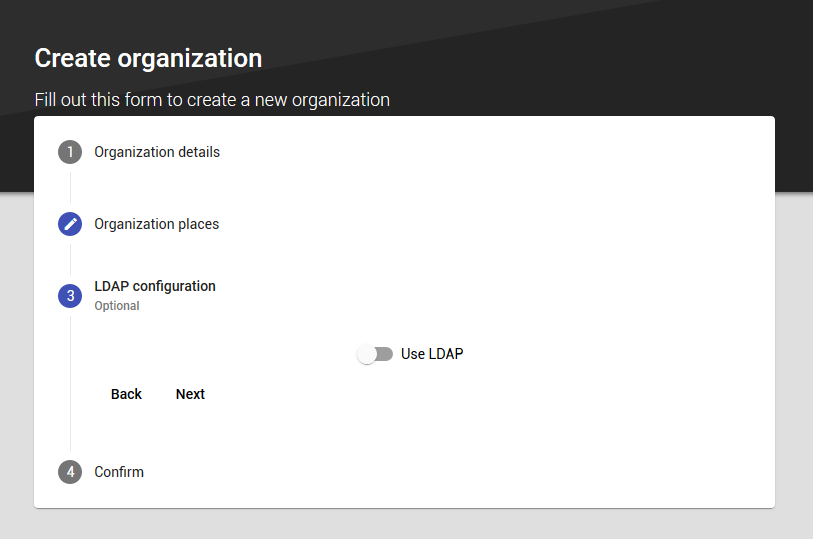
\includegraphics[width=120mm]{create-organization-3a.png}
      \caption{Configurazione LDAP non attiva}%
      \label{fig:web_app_configurazione_ldap_non_attiva}
    \end{figure}
    Inizialmente, la vista della pagina web presenta un \glossarioLocale{toggle} con la voce \textbf{Use LDAP} che è deselezionato, in quanto la configurazione LDAP è opzionale.
    Di default l'organizzazione è di dominio pubblico, ma se l'organizzazione che l'utente vuole creare è di dominio privato, allora deve cliccare sul toggle per attivare la visualizzazione dei campi che permettono la configurazione LDAP\@.
    \begin{figure}[H]
      \centering
      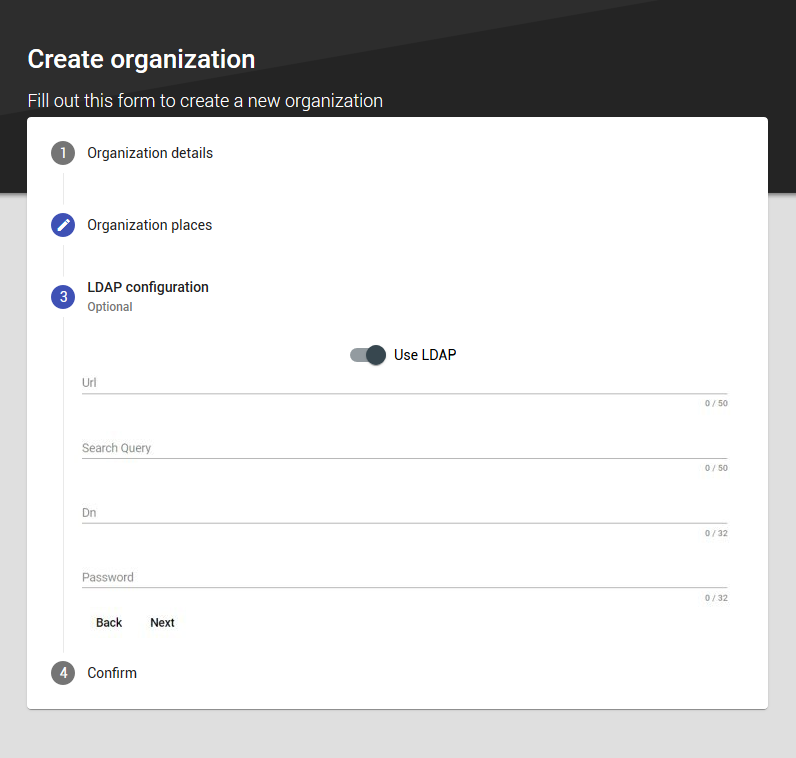
\includegraphics[width=120mm]{create-organization-3b.png}
      \caption{Inserimento dettagli configurazione LDAP}%
      \label{fig:web_app_inserimento_dettagli_configurazione_ldap}
    \end{figure}
    I campi che devono essere compilati sono:
    \begin{description}
      \item[Url:] che corrisponde all'indirizzo IP del server LDAP per l'autenticazione.
      \item[Domain Component:]  che corrisponde al dominio dell'organizzazione.
      \item[Common Name:] che è il nome distinto per accedere all'organizzazione privata.
      \item[Password:] che è la password per accedere all'organizzazione privata.
  \end{description}
    Cliccando \textbf{Back} si torna al passaggio 2, mentre cliccando \textbf{Next} si va al passaggio 4.

    \item \textbf{Confirm}

    \begin{figure}[H]
        \centering
        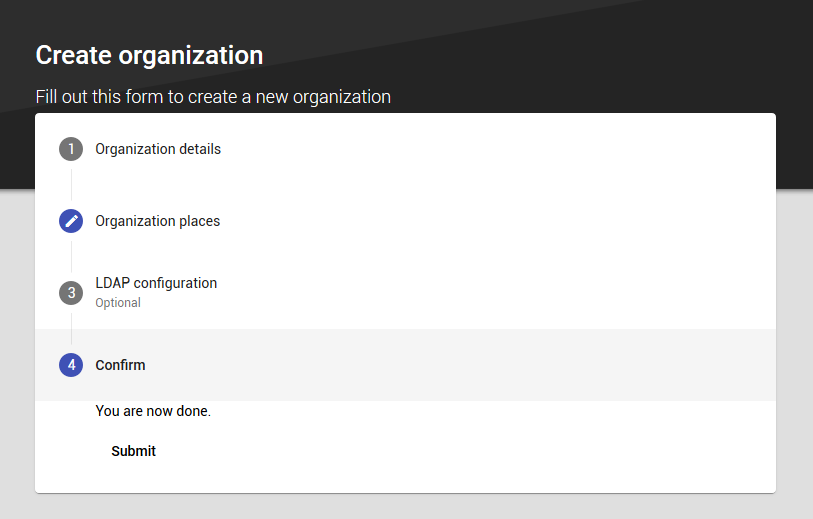
\includegraphics[width=120mm]{create-organization-4.png}
        \caption{Conferma creazione organizzazione}%
        \label{fig:web_app_conferma_organizzazione}
    \end{figure}
    Questo è l'ultimo passaggio per la conferma della creazione dell'organizzazione. Per confermarla, cliccare la voce \textbf{Submit}.
\end{enumerate}

\subsubsection{Modifica dettagli organizzazione}%
\label{subs:modififica_dettagli_organizzazione}

L'utente vuole modificare i dettagli di un'organizzazione, che avviene in 5 passaggi sequenziali.
I 5 passaggi per la modifica sono i seguenti:
\begin{enumerate}
    \item \textbf{Organization details}

    \begin{figure}[H]
        \centering
        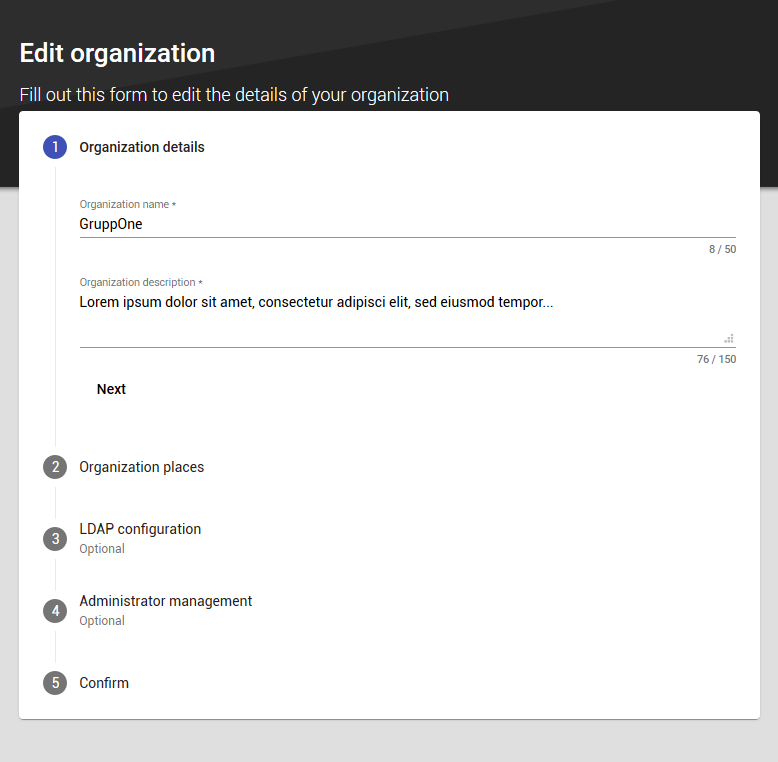
\includegraphics[width=120mm]{1-dettagli-organizzazione.png}
        \caption{Modifica dettagli dell'organizzazione}%
        \label{fig:web_app_modifica_dettagli_organizzazione}
    \end{figure}
    I campi che possono essere modificati sono:
    \begin{description}
        \item[Organization name:] che corrisponde al nome dell'organizzazione.
        \item[Organization description:] che corrisponde alla descrizione dell'organizzazione.
    \end{description}
    Cliccando \textbf{Next} si va al passaggio 2.

    \item \textbf{Organization places}

    \begin{figure}[H]
        \centering
        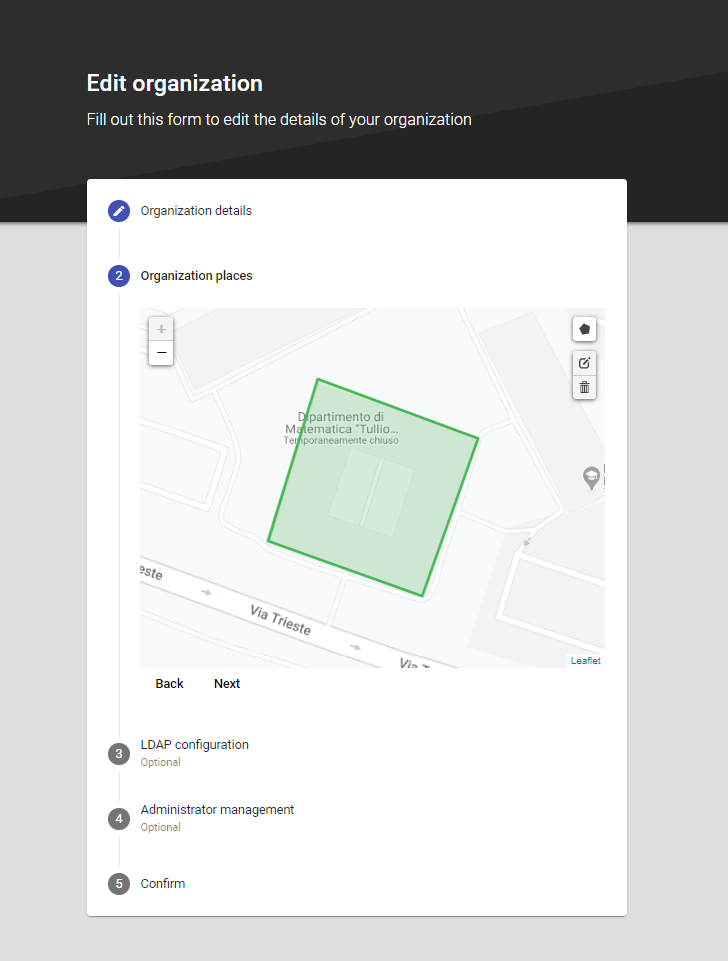
\includegraphics[width=120mm]{2-luoghi-organizzazione.png}
        \caption{Modifica luoghi dell'organizzazione}%
        \label{fig:web_app_modifica_luoghi_organizzazione}
    \end{figure}
    I luoghi si possono aggiungere, modificare ed eliminare direttamente dalla mappa interattiva, che si può ingrandire oppure rimpicciolire tramite i pulsanti in alto alla sinistra nella mappa.
    Per compiere azioni sulla mappa, ci sono tre pulsanti in alto a destra:
    \begin{itemize}
        \item cliccando il pulsante indicato con il poligono nero, si può creare un luogo bidimensionale sulla mappa cliccando con il tasto sinistro sui punti d'interesse. Per chiudere il poligono basta cliccare sul lato più adiacente all'ultimo punto cliccato dall'utente. Una volta creato il luogo, i dati relativi al luogo creato vengono rilevati attraverso \glossarioLocale{reverse geocoding}.
        \item cliccando il pulsante indicato con un foglio e una matita, si può modificare un luogo selezionandolo sulla mappa e modificando i vertici del poligono.
        \item cliccando il pulsante indicato con il cestino, si può eliminare un luogo selezionandolo sulla mappa.
    \end{itemize}
    Cliccando \textbf{Back} si torna al passaggio 1, mentre cliccando \textbf{Next} si va al passaggio 3.

    \item \textbf{LDAP configuration}~- \textit{opzionale}

    \begin{figure}[H]
        \centering
        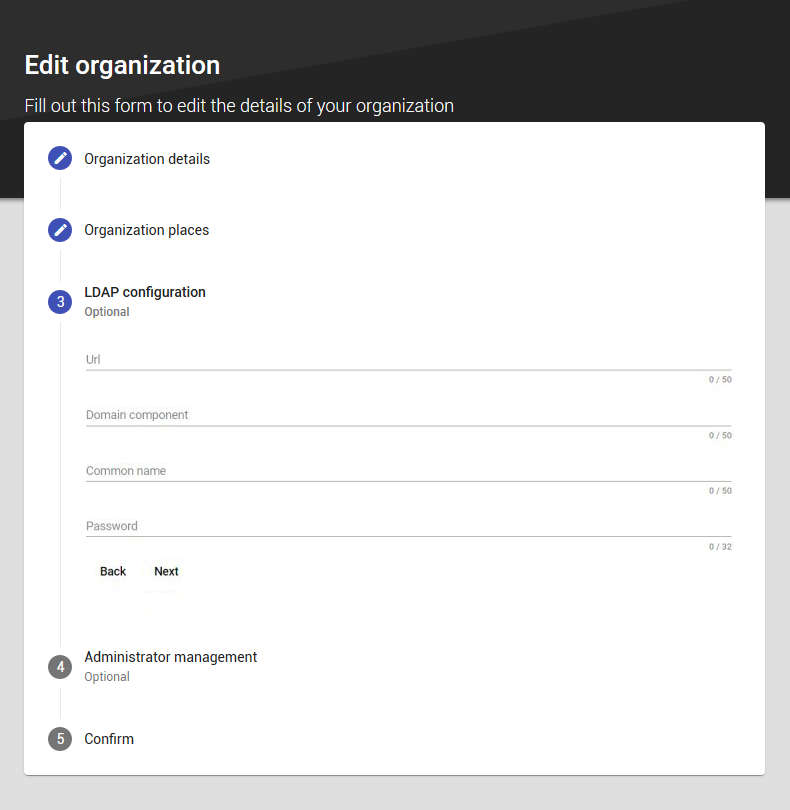
\includegraphics[width=120mm]{3-configurazione-ldap.png}
        \caption{Modifica configurazione LDAP}%
        \label{fig:web_app_modifica_configurazione_ldap}
    \end{figure}
    I campi che possono essere modificati sono:
    \begin{description}
      \item[Url:] che corrisponde all'indirizzo IP del server LDAP per l'autenticazione.
      \item[Domain Component:]  che corrisponde al dominio dell'organizzazione.
      \item[Common Name:] che è il nome distinto per accedere all'organizzazione privata.
      \item[Password:] che è la password per accedere all'organizzazione privata.
  \end{description}
    Cliccando \textbf{Back} si torna al passaggio 2, mentre cliccando \textbf{Next} si va al passaggio 4.

    \item \textbf{Administrator management}~- \textit{opzionale}

    \begin{figure}[H]
        \centering
        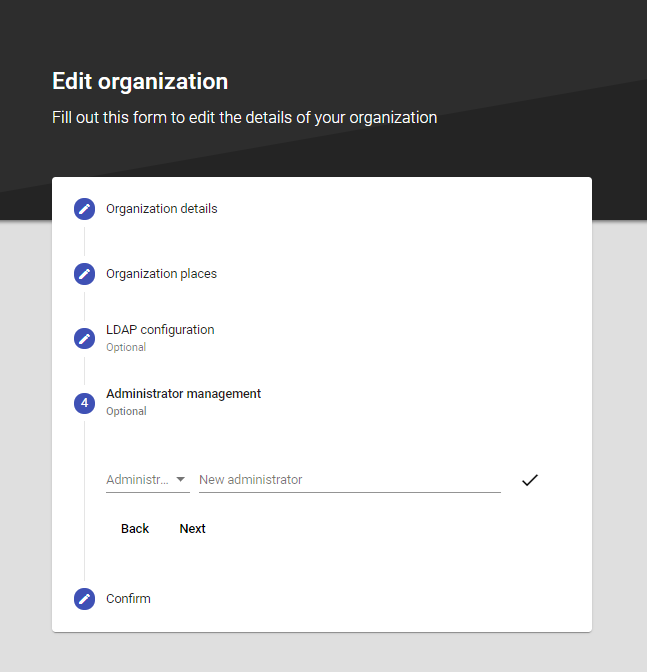
\includegraphics[width=120mm]{4-privilegi.png}
        \caption{Modifica privilegi utenti}%
        \label{fig:web_app_modifica_privilegi_utenti}
    \end{figure}
    Per aggiungere nuovi utenti con privilegi, si possono usufruire due campi di inserimento dati:
    \begin{itemize}
        \item un menu a tendina per la scelta della tipologia di utente, ovvero:
        \begin{itemize}
            \item \glossarioLocale{Manager}.
            \item \glossarioLocale{Viewer}.
        \end{itemize}
        \item un campo dove aggiungere l'email dell'utente del nuovo administrator.
    \end{itemize}
    Una volta che questi dati sono stati inseriti correttamente, l'utente con i nuovi privilegi viene aggiunto cliccando sulla spunta che si trova a destra dei campi d'inserimento.
    Non ci sono limiti per la ripetizione di questa procedura.
    Cliccando \textbf{Back} si torna al passaggio 3, mentre cliccando \textbf{Next} si va al passaggio 5.

    \item \textbf{Confirm}

    \begin{figure}[H]
        \centering
        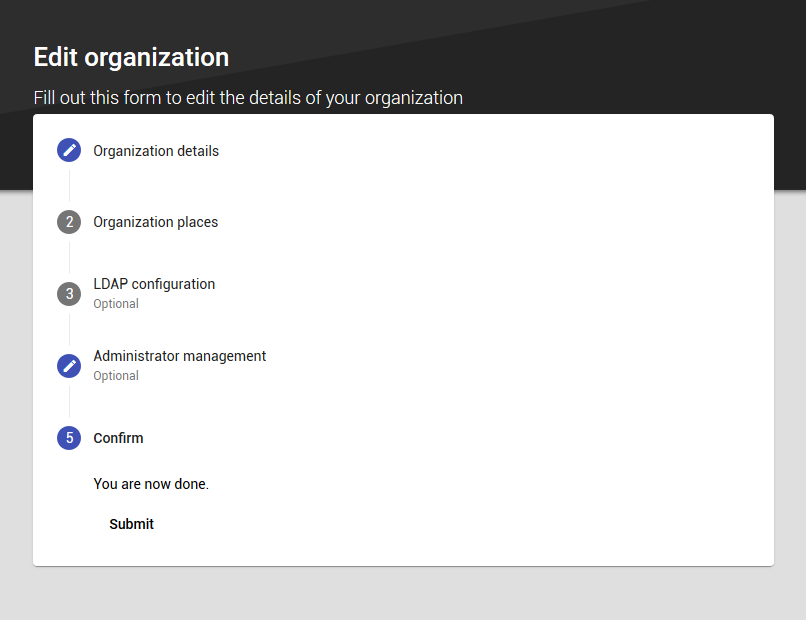
\includegraphics[width=120mm]{5-conferma-modifiche.png}
        \caption{Conferma modifiche}%
        \label{fig:web_app_conferma_modifiche}
    \end{figure}
    Questo è l'ultimo passaggio per la conferma delle modifiche effettuate. Per confermarle, cliccare la voce \textbf{Submit}.
\end{enumerate}

\subsubsection{Visualizza report organizzazione}%
\label{subs:visualizza_report_organizzazione}

\begin{figure}[H]
  \centering
  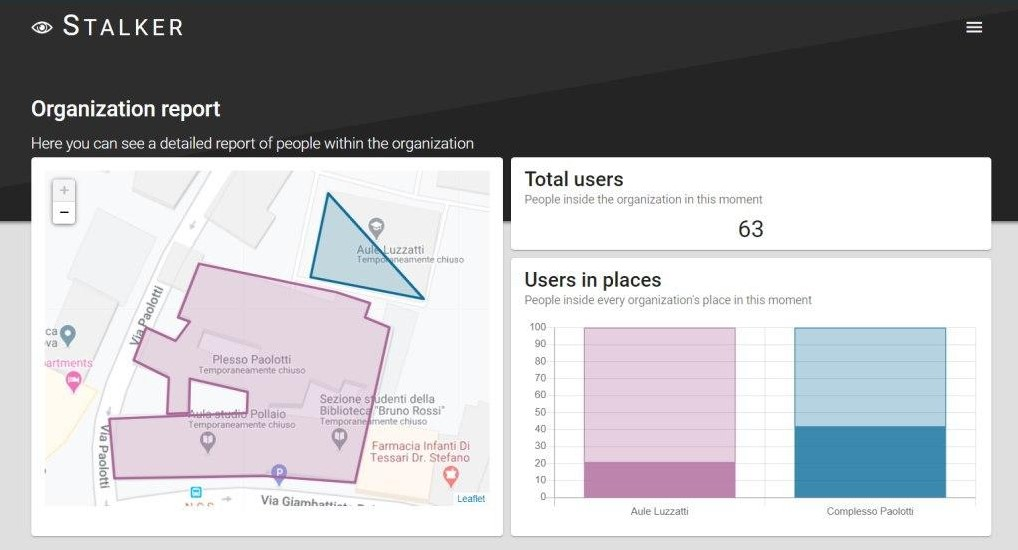
\includegraphics[width=180mm]{visualizza-report-organizzazione-1.jpg}
  \caption{Visualizza report organizzazione~- 1}%
  \label{fig:web_app_visualizza-report-organizzazione-1}
\end{figure}

L'utente ha la possibilità di visualizzare una serie di informazioni dettagliate relative ad un'organizzazione specifica.
Questa pagina contiene le seguenti informazioni:
\begin{itemize}
  \item la mappa a sinistra, che può essere ingrandita o rimpicciolita, mostra tutti i luoghi della specifica organizzazione.
  \item la finestra \textbf{Total users} mostra quanti utenti sono presenti attualmente nell'organizzazione.
  \item la finestra \textbf{Users in places} mostra un istogramma che indica nell'asse delle ascisse tutti i luoghi dell'organizzazione e nell'asse delle ordinate il numero di utenti attuali per ogni luogo dell'organizzazione. Da notare che il colore di ogni singola voce dell'istogramma ha lo stesso colore del corrispondente luogo indicato sulla mappa.
  \begin{figure}[H]
    \centering
    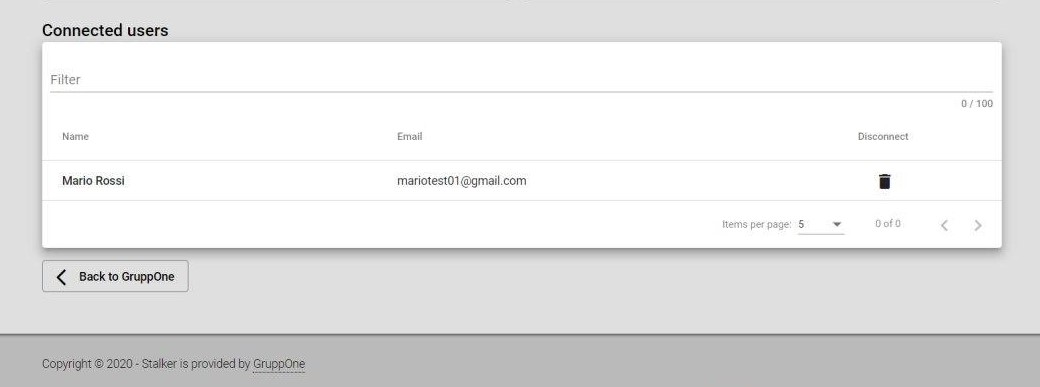
\includegraphics[width=180mm]{visualizza-report-organizzazione-2.jpg}
    \caption{Visualizza report organizzazione~- 2}%
    \label{fig:web_app_visualizza-report-organizzazione-2}
  \end{figure}
  \item la finestra \textbf{Connected users} mostra tutti gli utenti connessi attualmente all'organizzazione.
  Ogni utente è caratterizzato dalle seguenti informazioni:
  \begin{description}
    \item[Name:] nome e cognome dell'utente.
    \item[Email:] email dell'utente.
  \end{description}
  L'utente ha la possibilità di interagire con la finestra e può eseguire queste operazioni:
  \begin{itemize}
    \item selezionare un utente dalla lista degli utenti connessi per accedere al report personale (sotto-sezione §~\ref{subs:visualizza_report_utente}).
    \item disconnettere un utente da Stalker, cliccando il pulsante a forma di bidone posto sotto la colonna \textbf{Disconnect}. Una volta cliccato, uscirà un pop-up per confermare o annullare l'operazione.
    \item filtrare gli utenti in lista per nome e cognome tramite un'apposita area di ricerca indicata con il placeholder \textit{Filter}, sopra la lista degli utenti.
    \item filtrare il numero di utenti visualizzabili in una pagina, tramite la tendina \textit{Items per page} sotto la lista degli utenti.
    \item cambiare la pagina della lista degli utenti, tramite le apposite frecce direzionali sotto la lista degli utenti.
    \item tornare alla pagina precedente cliccando sul pulsante \textbf{Back to GruppOne} posto sotto la finestra \textit{Connected users}.
  \end{itemize}
\end{itemize}

\subsubsection{Visualizza report utente}%
\label{subs:visualizza_report_utente}

\begin{figure}[H]
  \centering
  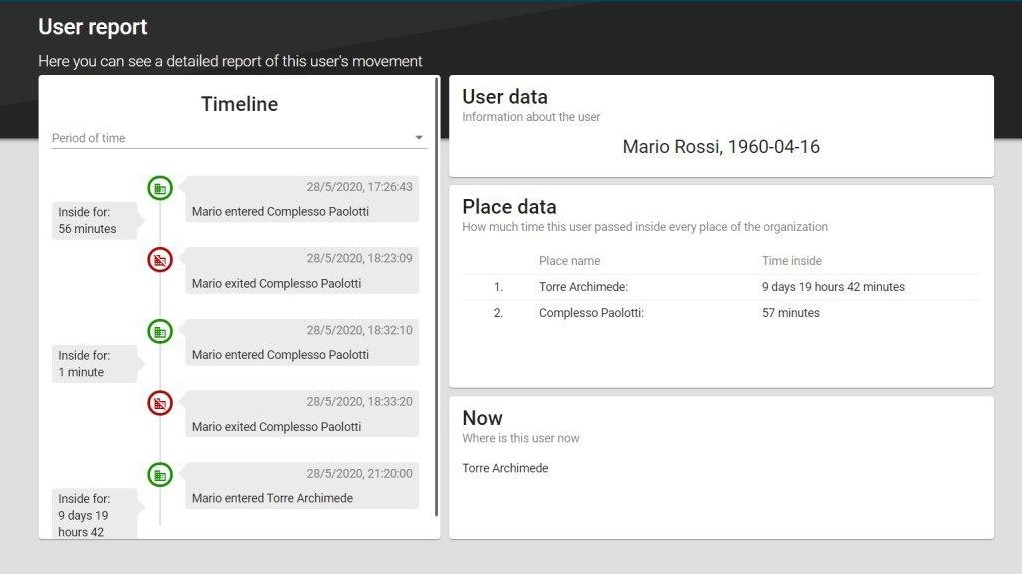
\includegraphics[width=180mm]{visualizza-report-utente.jpg}
  \caption{Visualizza report utente}%
  \label{fig:web_app_visualizza-report-utente}
\end{figure}
L'utente ha la possibilità di visualizzare una serie di informazioni dettagliate relative ad un utente selezionato, che è attualmente connesso ad un luogo dell'organizzazione corrente.
Questa pagina contiene le seguenti informazioni:
\begin{itemize}
  \item la finestra \textbf{Timeline} indica l'intero storico dei movimenti dell'utente selezionato all'interno dell'organizzazione corrente, specificando data e ora di entrata ed uscita da un determinato luogo e il tempo di permanenza. È possibile selezionare un'intervallo di tempo tramite il menu a tendina \textbf{Period of time}.
  \item la finestra \textbf{User data} indica le informazioni principali dell'utente selezionato, ovvero:
  \begin{itemize}
    \item nome.
    \item cognome.
    \item data di nascita.
  \end{itemize}
  \item la finestra \textbf{Place data} indica in una tabella quanto tempo ha passato l'utente selezionato all'interno di ogni luogo nell'organizzazione corrente. Ogni riga è composta dal nome del luogo (colonna \textbf{Place name}) e dal tempo di permanenza totale all'interno di ogni luogo (colonna \textbf{Time inside}).
  \item la finestra \textbf{Now} indica in quale luogo si trova attualmente l'utente selezionato.
\end{itemize}
L'utente può tornare alla pagina precedente cliccando sul pulsante \textbf{Back to GruppOne} posto a fine pagina. %TODO verificare se c'è nella pagina: in caso affermativo aggiornare l'img, altrimenti cancellare questa frase.

\subsection{Risoluzione dei problemi}%
\label{subs:web_app_risoluzione_problemi}

\subsubsection{Accesso all'applicazione non disponibile}%
\label{subs:web_app_accesso_non_disponibile}

Nel caso si verifichino problemi di collegamento alla web application, visitare il sito \href{http://www.isitdownrightnow.com/}{http://www.isitdownrightnow.com/} per verificare se il problema è legato alla web application di Stalker.
Nel caso la risposta sia affermativa, segnalarlo nelle modalità discusse nella sezione §~\ref{sec:supporto_tecnico}.

\end{document}
